% 05-Metodologia_Presentacion_Tesis.tex
% Diapositivas de la sección Metodología

\section{Metodología}

\begin{frame}
\frametitle{Flujo General de la Metodología}
\begin{itemize}
    \item Desarrollo de modelos de aprendizaje profundo para la detección de 15 patologías pulmonares en rayos X.
    \item Dos enfoques principales: ResNet50 (CNN) y Vision Transformer (ViT).
    \item Proceso estructurado: preprocesamiento, entrenamiento, evaluación y extensión a nuevas patologías.
\end{itemize}
\end{frame}

\begin{frame}
\frametitle{Bases de Datos y Composición}
\begin{itemize}
    \item Uso del dataset ChestX-ray14 (112,120 imágenes, 30,805 pacientes, 14 patologías).
    \begin{itemize}
        \item National Institutes of Health (NIH)
    \end{itemize}
    \item Extensión con imágenes de COVID-19 y saludables.
    \begin{itemize}
        \item bimcv-covid19. Banco de Imágenes Médicas de la Comunidad Valenciana (BIMCV)
        \item covid-chestxray-dataset. Universidad de Montreal
    \end{itemize}
    \item Re-etiquetado de datos usando modelos automáticos para mejorar la calidad de las etiquetas.
\end{itemize}
\end{frame}

\begin{frame}
    \frametitle{Composición del Dataset por Patología}
    \begin{table}[!ht]
        \centering
        \fontsize{7}{8}\selectfont
        \begin{tabular}{| r |l | c | c | c |}
         \hline
         Clase & Patología & Fuente & Entrenamiento & Prueba  \\
         \hline\hline
         1  & Cardiomegaly       & 1 & 5897  & 1069 \\
         2  & Emphysema          & 1 & 3496  & 1093 \\
         3  & Effusion           & 1 & 13737 & 4658 \\
         4  & Hernia             & 1 & 4470  & 86   \\
         5  & Infiltration       & 1 & 17122 & 6112 \\
         6  & Mass               & 1 & 7862  & 1748 \\
         7  & Nodule             & 1 & 9250  & 1623 \\
         8  & Atelectasis        & 1 & 13762 & 3279 \\
         9  & Pneumothorax       & 1 & 6303  & 2665 \\
         10 & Pleural-Thick.     & 1 & 8022  & 1143 \\
         11 & Pneumonia          & 1 & 6031  & 555  \\
         12 & Fibrosis           & 1 & 9072  & 435  \\
         13 & Edema              & 1 & 6953  & 925  \\
         14 & Consolidation      & 1 & 9796  & 1815 \\
         ---&  Healthy           & 1 & 35645 & 9861 \\
         \hline
         11 & Pneumonia          & 2 & 5475  & 594  \\
         15 & COVID-19           & 2 & 2873  & 1904 \\
         ---&  Healthy           & 2 & 8661  & 1926 \\
         \hline
        \end{tabular}
        \caption{Número de radiografías de pecho por patología en el conjunto de datos. Fuentes (DS): (1) ChestX-ray14,
                 (2) BIMCV-COVID19 y covid-chestxray-dataset. Pleural-Thick. es una abreviación para Pleural-Thickening.}
        \label{table_dataset}
    \end{table}
\end{frame}

\begin{frame}
\frametitle{Preprocesamiento de Imágenes}
\begin{itemize}
    \item Redimensionamiento a $1024 \times 1024$ y $384 \times 384$ píxeles según el modelo.
    \item Ecualización por histograma sobre el canal Y en el espacio de color YUV.
    \item Normalización (media y std de ImageNet) para cada canal RGB.
    \item Data augmentation: flip horizontal.
\end{itemize}
\end{frame}

\begin{frame}
\frametitle{Arquitectura de los Modelos}
    \textbf{Modelo CNN}
    \begin{itemize}
        \item Basado en \textit{CheXNet}.
        \begin{itemize}
            \item Backbone \textit{DenseNet121} con 121 capas.
            \item Pre-entrenado en ImageNet.
            \item Capa de clasificación con 14 clases.
        \end{itemize}
        \item Propuesta construida con:
        \begin{itemize}
            \item Backbone \textit{ResNet50} con 50 capas.
            \item Pre-entrenado en ImageNet.
            \item MLP network de clasificación con 15 clases.
        \end{itemize}
    \end{itemize}
\end{frame}

\begin{frame}
\frametitle{Arquitectura de los Modelos}
\begin{table}[!ht]
    \centering
    \begin{tabular}{| l|c | c | r |}
    \hline
                 &     Input   &  Output    &  \\
    Layer        &   dimension & dimension  & Parameters \\
    \hline\hline
    ResNet50     &     3,1024,1024 &     2048,1,1 & 24,036,431 \\
    Flatten      &     2048        &     2048     &  --        \\
    Dense        &     2048        &     256      & 524,544    \\
    ReLU         &     256         &     256      & --         \\
    Drop-0.25  &     256         &     256      & --         \\
    Dense        &     256         &     15       &  3,855     \\
    Sigmoid      &     15          &     15       & --         \\
    \hline
    \end{tabular}
    \caption{Arquitectura de la red neuronal usada en el modelo propuesto basado en ResNet50. Las capas
    densas incluyen el término de bias. \textit{Drop-0.25} significa una capa \textit{Dropout} con
    probabilidad de 0.25.}
    \label{table_resnet50}
\end{table}
\end{frame}

\begin{frame}
\frametitle{Arquitectura de los Modelos}
    \textbf{Modelo ViT}
    \begin{itemize}
        \item Basado en \textit{ViT}.
        \begin{itemize}
            \item Backbone \textit{ViT-L/32-384 BERT}.
            \item Pre-entrenado en ImageNet.
            \item MLP network de clasificación con 15 clases.
        \end{itemize}
    \end{itemize}
\end{frame}

\begin{frame}
\frametitle{Arquitectura de los Modelos}
\begin{table}[!ht]
    \centering
    \begin{tabular}{| l | c |}
     \hline
    \textbf{Input size}  & 384 $\times$ 384 \\
    \textbf{Patch size}  & 32 $\times$ 32 \\
    \textbf{Layers}      & 12  \\
    \textbf{Hidden size} & 768 \\
    \textbf{MLP Size}    & 3072 \\
    \textbf{Heads}       & 12 \\
    \textbf{Params}      & 87M \\
     \hline
    \end{tabular}
    \caption{Configuración de la arquitectura del modelo ViT usado. Usa imágenes de tamaño
             $384 \times 384$ con 3 canales correspondientes al modo RGB. En total cuenta con 12
             cabezas de atención y 12 codificadores internos.}
\label{table_ViTBase}
\end{table}
\end{frame}

\begin{frame}
\frametitle{Arquitectura de los Modelos}
\begin{figure}[ht!]
    \centering
    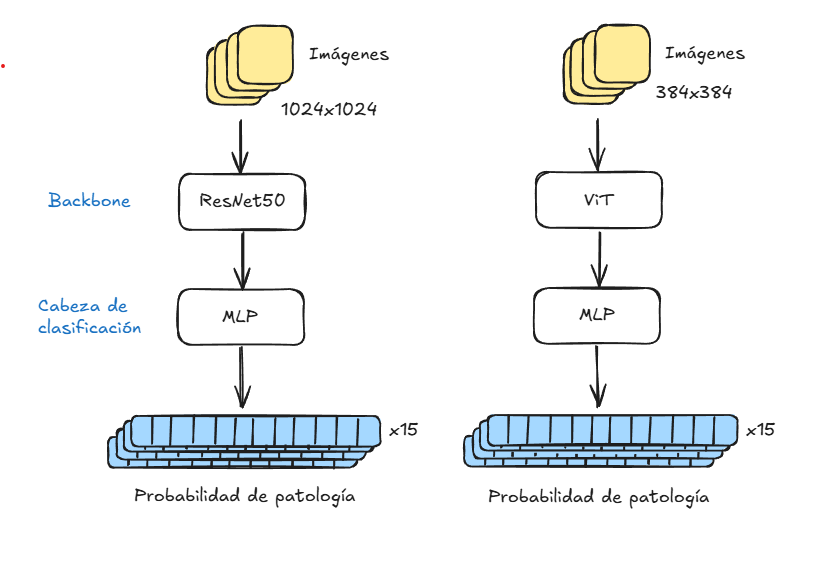
\includegraphics[width=0.6\textwidth]{./images/models.png}
    \caption{Representación de la arquitectura de los modelos basados en ResNet50 y ViT.}
\end{figure}
\end{frame}

\begin{frame}
\frametitle{Función de Coste}
\begin{itemize}
    \item Función de pérdida basada en \textit{Binary Cross-Entropy} ponderada.
    \item Soluciona el desbalanceamiento de clases en el dataset.
    \item Pesos inversamente proporcionales al número de casos por clase.
\end{itemize}

\begin{equation}
    L(\hat y, y) = \sum_{c=0}^{15} \left[ w_c^{(p)} y_c \log \hat y_c + w_c^{(n)} (1-y_c) \log (1- \hat y_c) \right]
\end{equation}

\begin{equation}
    w_c^{(n)} = \frac{n_c}{N} \;\;\;\; \text{y} \;\;\;\; w_c^{(p)} = 1-  w_c^{(n)}
\end{equation}

\small
donde $y$ es el vector de etiquetas reales, $\hat{y}$ las predicciones, $w_c^{(p)}$ y $w_c^{(n)}$ son los pesos para casos positivos y negativos de la clase $c$, $N$ es el tamaño del dataset y $n_c$ el número de casos de la clase $c$.
\end{frame}

\begin{frame}
\frametitle{Entrenamiento: Transfer Learning y Fine-Tuning}
\begin{itemize}
    \item \textbf{Etapa 1 - Entrenamiento Inicial}
    \begin{itemize}
        \item Backbone congelado, solo se entrena el clasificador MLP
        \item ResNet50: 35 épocas, ViT: 25 épocas
    \end{itemize}
    \item \textbf{Etapa 2 - Fine-tuning}
    \begin{itemize}
        \item Descongelamiento de últimas capas del backbone
        \item ResNet50: último bloque convolucional (20 épocas)
        \item ViT: dos últimos bloques Transformer (12 épocas)
    \end{itemize}
    \item \textbf{Etapa 3 - Full-tuning}
    \begin{itemize}
        \item Entrenamiento completo de toda la red
        \item ResNet50: 10 épocas, ViT: 8 épocas
    \end{itemize}
    \item \textbf{Configuración}
    \begin{itemize}
        \item Optimizador: Adam (ResNet50: LR=1e-4, ViT: LR=1e-5)
        \item Parámetros de inercia: $\beta_1=0.9$, $\beta_2=0.999$ y LR decay: 0.1
        \item Umbral de mejora: $1\times 10^{-4}$ (plateau escape) 10 it.
        \item Data augmentation: flip horizontal (p=0.5)
    \end{itemize}
\end{itemize}
\end{frame}

\begin{frame}
\frametitle{Extensión y Generalización}
\begin{itemize}
    \item El modelo puede ser extendido fácilmente a nuevas patologías (ejemplo: tuberculosis).
    \item El proceso de re-etiquetado y entrenamiento permite adaptar el sistema a diferentes escenarios clínicos.
    \item Resultados competitivos frente al estado del arte en todas las patologías evaluadas.
\end{itemize}
\end{frame}

\begin{frame}
\frametitle{Extensión a Tuberculosis - Dataset}
\begin{itemize}
    \item \textbf{Propósito}: Demostrar capacidad de extensión del modelo
    \begin{itemize}
        \item Clasificador binario para tuberculosis pulmonar
        \item Enfermedad bacteriana común en países en desarrollo
        \item Frecuente en pacientes con VIH/SIDA
    \end{itemize}
    \item \textbf{Composición del dataset}
    \begin{itemize}
        \item Entrenamiento: 888 casos positivos, 6,000 negativos
        \item Prueba: 488 casos positivos, 1,600 negativos
    \end{itemize}
    \item \textbf{Fuentes de datos}
    \begin{itemize}
        \item TBX11K dataset, India (DA and DB) dataset
        \item Montgomery County dataset, Shenzhen Hospital dataset
    \end{itemize}
    \item \textbf{Nota}: Casos 'no tuberculosis' incluyen pacientes saludables y con otras afecciones
\end{itemize}
\end{frame}

\begin{frame}
\frametitle{Extensión a Tuberculosis - Arquitectura}
\begin{itemize}
    \item \textbf{Estrategia}: Transfer learning eficiente
    \begin{itemize}
        \item Backbone ResNet50 pre-entrenado (pesos congelados)
        \item Rama adicional específica para tuberculosis
    \end{itemize}
    \item \textbf{Rama de clasificación}
    \begin{itemize}
        \item Dense: 256 $\rightarrow$ 128 dimensiones
        \item ReLU + Dropout (p=0.20)
        \item Dense: 128 $\rightarrow$ 1 (Sigmoid)
    \end{itemize}
    \item \textbf{Ventajas}
    \begin{itemize}
        \item Mantiene detección de 15 patologías originales
        \item Agrega tuberculosis como salida binaria adicional
        \item Solo entrena nuevas capas densas
        \item Conserva conocimiento previamente adquirido
    \end{itemize}
\end{itemize}
\end{frame}

\begin{frame}
\frametitle{Extensión a Tuberculosis - Arquitectura}
\begin{figure}[ht!]
    \centering
    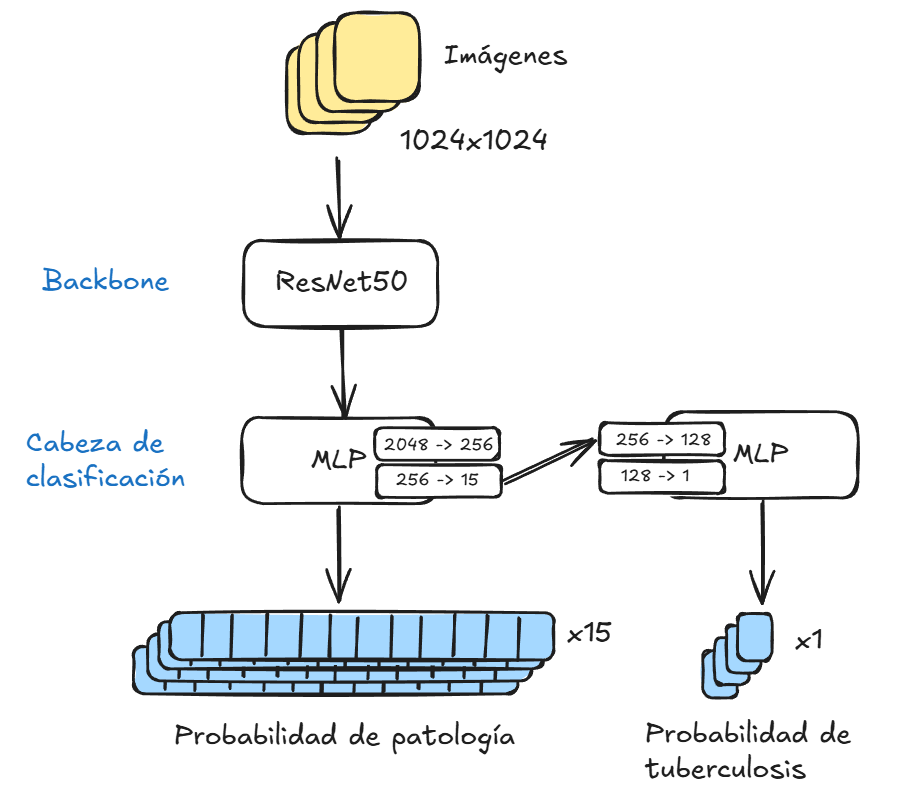
\includegraphics[width=0.5\textwidth]{./images/model-tub.png}
    \caption{Representación de la arquitectura de extensión a tuberculosis.}
\end{figure}
\end{frame}

\begin{frame}
\frametitle{Extensión a Tuberculosis - Entrenamiento y Resultados}
\begin{itemize}
    \item \textbf{Entrenamiento}
    \begin{itemize}
        \item Estrategia de entrenamiento inicial
        \item Backbone congelado, solo nuevas capas densas
        \item Misma función de pérdida ponderada y optimizador Adam
    \end{itemize}
    \item \textbf{Resultados}
    \begin{itemize}
        \item F1-score: 0.707, Accuracy: 0.846
        \item 388 verdaderos positivos de 488 casos
        \item Comparable con métodos específicos de la literatura
    \end{itemize}
    \item \textbf{Análisis adicional}
    \begin{itemize}
        \item Modelo original detecta tuberculosis como COVID-19/neumonía
        \item Características radiológicas similares entre patologías
        \item Confirma necesidad de entrenamiento específico
    \end{itemize}
\end{itemize}
\end{frame}


\begin{frame}
\frametitle{Evaluación y Métricas}
\begin{itemize}
    \item \textbf{Configuración de evaluación}
    \begin{itemize}
        \item Conjunto de prueba independiente (estructura original ChestX-ray14)
        \item Umbral de clasificación: 0.5 para todas las patologías
    \end{itemize}
    \item \textbf{Métricas principales}
    \begin{itemize}
        \item AUC-ROC: Capacidad discriminativa del modelo
        \item AUC-PR: Especialmente importante para clases desbalanceadas
        \item F1-Score: Balance entre precisión y recall
        \item Accuracy: Proporción de predicciones correctas
    \end{itemize}
    \item \textbf{Resultados destacados}
    \begin{itemize}
        \item ResNet50: AUC-ROC Global-15 = 0.852 (supera CheXNet: 0.841)
        \item COVID-19 ROC AUC: ResNet50 (0.991), ViT (0.982)
        \item Supera a radiólogos en 6/15 patologías
    \end{itemize}
    \item \textbf{Visualizaciones}
    \begin{itemize}
        \item Curvas ROC: TPR vs FPR por patología
        \item GradCAM: Regiones de atención del modelo
        \item Matrices de confusión: TP, TN, FP, FN
    \end{itemize}
\end{itemize}
\end{frame}
